\documentclass[pageno]{jpaper}

%replace XXX with the submission number you are given from the ISCA submission site.
\newcommand{\IWreport}{2015}

\usepackage[normalem]{ulem}
\usepackage{graphicx}
\usepackage{caption}
\usepackage{subcaption}
\usepackage{listings}
\usepackage{xcolor}
\lstset { %
    language=C++,
    backgroundcolor=\color{black!5}, % set backgroundcolor
    basicstyle=\ttfamily
}
\lstMakeShortInline[]|

\graphicspath{{./figures/}}

\begin{document}

\title{Virtual Reality 3D Scanning}

\date{}
\maketitle

\thispagestyle{empty}

\begin{abstract}
  We propose a head-mounted device and accompanying software for 3D scanning of
  a static scene that provides real-time feedback during scanning. This method
  allows viewing the current scan from multiple angles and viewpoints, while also
  providing a feeling of presence through a virtual reality interface. Holes and
  other artifacts can be immediately identified and fixed interactively. Further,
  the device supports position and rotation tracking which allows for registration
  of multiple scans at interactive speeds.
\end{abstract}

\section{Introduction}

\ldots

\section{Related Work}

\ldots

\section{Methodology}

\subsection{Live point cloud view}
\label{sec:live-view}

The most basic element of the device is a live display of the depth camera feed
in a virtual reality view. The view can be rotated and zoomed in and out of with
the mouse. The device runs at very low latency (achieving about 60 frames per
second).

\begin{figure}
  \centering
    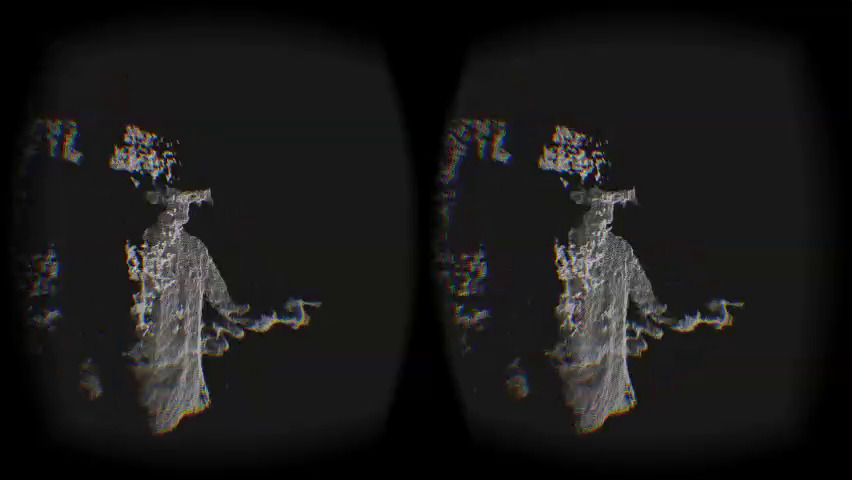
\includegraphics[width=0.62\textwidth]{shot2.png}
  \caption{Live point cloud view}
  \label{fig:live-view}
\end{figure}

Figure~\ref{fig:live-view} shows the virtual reality render of a user viewing a
live point cloud capture of oneself. In this case the depth camera has been
mounted on a table in front of the user simply for the purpose of the
example. The user can move around and see the point cloud update in real-time,
while the movement of the head also moves and re-orients the viewpoint providing
immersion.

\subsection{First-person view}

When the depth camera is mounted on the head-mounted virtual reality display and
the point clouds read from it are transformed by the eye transform given by the
display, a first person view effect is achieved. This is because during
rendering the view transform is used, which is the inverse of the eye transform,
having the point cloud data in the space of the depth camera go to identity in
camera space during rendering.

As before, this view is real-time, and so effectively this becomes a 3D
`see-through' display of the environment in point cloud form. The user can
switch between first person view and the third-person mode with mouse control
described in the earlier section at any time. The third-person mode allows
discovering holes easily (since they are often better visible at right angles to
the eye vector), while the first person view allows the user to position and
orient the head-mounted display for effective scanning in a more intuitive
fashion once the holes are found.

Figure~\ref{fig:first-person-view} shows such a first person display. The hand
of the user can be seen along with the interior of a room in the background.

\begin{figure}
  \centering
    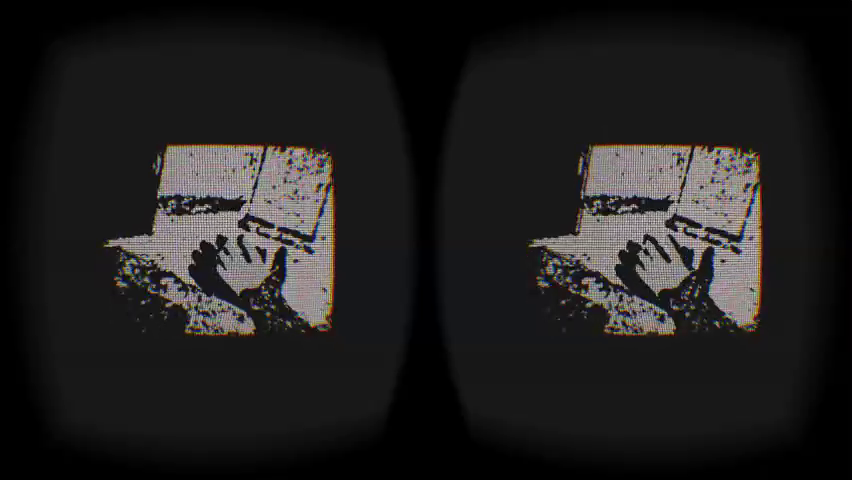
\includegraphics[width=0.62\textwidth]{shot1.png}
  \caption{First person view}
  \label{fig:first-person-view}
\end{figure}

\subsection{Live registration}

Point cloud registration is the process of placing multiple point cloud captures
so that their relative positions and orientations correspond to the real-world
relative positions and orientations of the surfaces that they capture. With no
information on the placement of the camera when the picture was taken this is a
hard problem since the point clouds must be analyzed for possible
overlaps. However, since the depth camera is mounted on a head-mounted device
that has its position and orientation tracked, we can use this information to
place the point cloud captures. This allows registration at interactive speeds,
provided the location of the camera relative to the location of the origin in
the head-mounted device frame is properly accounted for.

Figure~\ref{fig:registration} shows multiple frames of a quick swipe of the
head-mounted depth camera setup across the wall of a room with a window and a
bed, as seen from a static third-person viewpoint. The union of the frames is
not displayed, but their relative positions are such that their union should
give the structure of the scanned portion of the room.

\begin{figure}
  \centering
  \begin{subfigure}[b]{0.3\textwidth}
    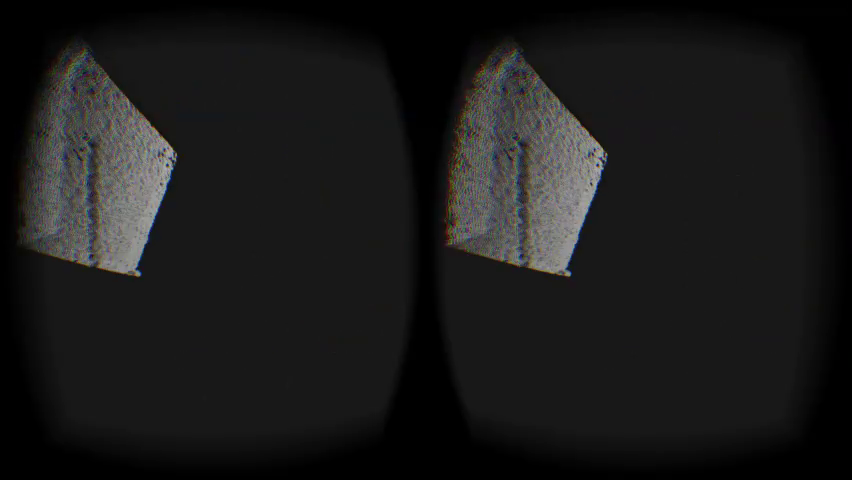
\includegraphics[width=\textwidth]{shot3.png}
    \label{fig:gull}
  \end{subfigure}%
  \qquad
  \begin{subfigure}[b]{0.3\textwidth}
    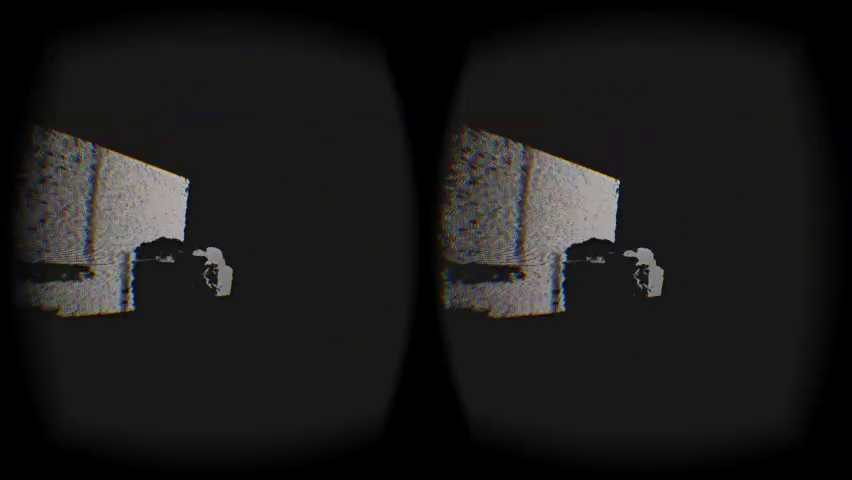
\includegraphics[width=\textwidth]{shot4.png}
    \label{fig:tiger}
  \end{subfigure}
  \qquad
  \begin{subfigure}[b]{0.3\textwidth}
    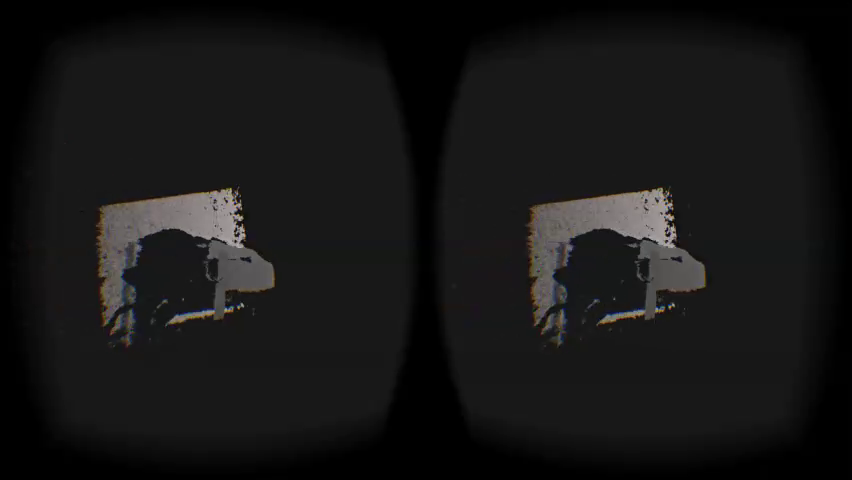
\includegraphics[width=\textwidth]{shot5.png}
    \label{fig:mouse}
  \end{subfigure}
  \qquad
  \begin{subfigure}[b]{0.3\textwidth}
    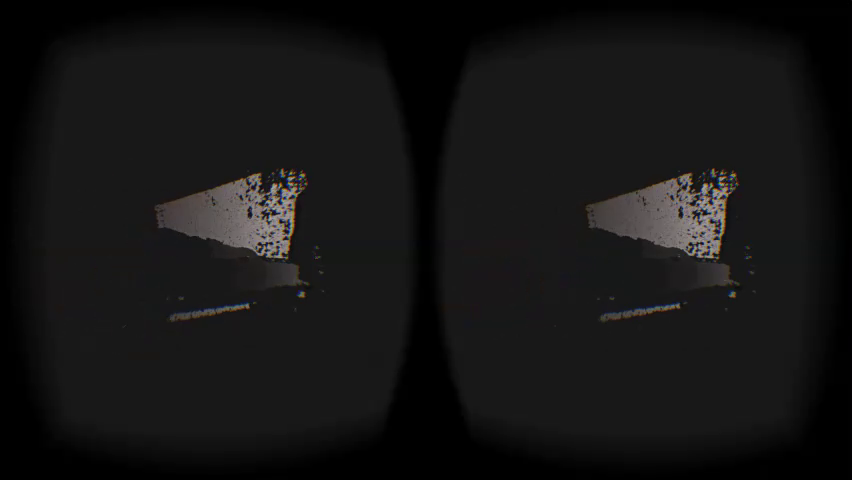
\includegraphics[width=\textwidth]{shot6.png}
    \label{fig:mouse}
  \end{subfigure}
  \caption{Live registration of multiple captures}\label{fig:animals}
  \label{fig:registration}
\end{figure}

\section{Implementation}

The program was written in C++, using C++11 features such as lambdas. It uses
OpenGL for rendering, SimpleDirectMedia Layer (SDL) to create a window and
maintain an OpenGL context, the Oculus Rift SDK to render to the Oculus Rift and
read position/rotation tracking data, the OpenGL Mathematics (GLM) library for
mathematical structures and operations and the Intel Double Springs 4 SDK to
read depth images from the Intel Double Springs 4 camera.

The implementation is divided into 4 main systems, each represented by a class:
|Game|, |VR|, |DS|, |Scene|. |Game| runs the main event loop, |VR| handles
virtual reality rendering, |DS| reads depth camera data and |Scene| manages
scene elements and draws them.

\subsection{\lstinline|Game|}

|Game| maintains an SDL window with an OpenGL context, listens for events and
notifies event handlers, and provides a frames-per-second display. The
constructor initializes SDL, creates a window and an OpenGL context, and the
destructor quits SDL.

In its public interface, the most important part of |Game| is the
|Game::update(update, draw)| method, which runs the main event loop, taking two
functions |update| and |draw|. The |update| function is called every loop, and
the |draw| function is called whenever the scene must be re-rendered. These are
separate callbacks to allow updating at a higher frequency than drawing, or to
allow update even when not drawing, such as when the window is minimized.

Other than this, |Game| provides methods to retrieve the SDL window, access
command-line arguments and quit the program.

\subsection{\lstinline|VR|}

|VR| is the main interface to the virtual reality display. It uses the Oculus
Rift SDK to communicate with the Oculus Rift device, and the implementation has
been designed so there are no references to the Oculus Rift SDK elsewhere in the
code and where required the device is communicated with only through the |VR|
class. The constructor creates an OpenGL framebuffer to render to that is shared
with the Oculus SDK, resizes and repositions the window to render to the Oculus
Rift, and enables position and rotation tracking. The destructor deinitializes
all of this.

The public |VR::draw(drawer)| method draws to the virtual reality display,
taking a function |drawer| that draws the actual scene as if drawing to a
conventional screen. It achieves this by calling |drawer| twice, once for each
eye, each time setting up the projection and view matrices according to the eye
rendered from. The view matrix is dependent upon the position and rotation of
the head-mounted display and takes into account the displacement of each eye
from the center of the head. To calculate the view matrix it computes the
inverse of the matrices returned by |VR::eye_transforms()|.

The public |VR::eye_transforms()| returns two matrices in an |std::array|, each
representing the camera matrix of an eye. It also supports an optional boolean
parameter |mid|. If |mid| is true, it returns the camera matrix of the `mid' eye,
as if viewing the scene from the center of the head with the same eye
orientation.

\subsection{\lstinline|DS|}

|DS| is the main interface to the depth camera. It uses the Intel Double Springs
4 SDK to communicate with the Intel Double Springs 4 depth camera. The
constructor probes for the depth camera configuration, enables Z (depth) capture
and sets the camera resolution to 480x360.

The public |DS::points()| method captures a depth image from the camera and
returns an |std::vector| representing a point cloud. These points are placed in
the camera-space of the depth camera, with the $z$-axis pointing forward, the
$x$ axis pointing right and the $y$ axis pointing up, in a frame that looks
`down' through the camera.

\subsection{\lstinline|Scene|}

|Scene| handles the maintenance and drawing of scene elements. In the current
implementation, there are no scene elements other than the point cloud
itself. The scene can be rotated and zoomed in and out of with the mouse. The
|Scene::update()| function must be called every update to handle mouse
events. |Scene::draw(points, vr)| draws the point cloud, taking the array of
points |points| and the current |VR| instance |vr|. The |VR| instance is
required so that the points can be placed in their correct world-space position
using the `mid' eye camera matrix returned by |VR::eye_transforms()|. Since the
depth camera is attached to the front of the head-mounted display, this achieves
the effect of registering multiple captures from the depth camera.

\section{Future Work}

\subsection{Color capture}

This would be a simple addition to the existing implementation. The current
implementation only stores positions of points and not their color. Adding color
would provide a more complete rendering of the scene captured. The Intel Double
Springs 4 camera has a `third eye' that takes standard color images of the
scene. It provides an interface to find coordiantes in the third image
corresponding to those in depth images. By creating an OpenGL texture with the
third image as its data and providing a UV transform, we can add color to the
point cloud in an efficient manner. This texture-mapping based approach would
also translate well in case of mesh surface reconstructions from the depth
image.

Adding color capture would involve very minimal effort and could be accomplished
within the span of a couple days and at most one week.

\subsection{Research more related work}

This paper has focused more on approach and implementation than related work in
the field. Some of the related work includes Kintinuous (which extends the
registration features of Kinect cameras to much larger spaces) and AR-Rift
(which displays first person video of the real world in Oculus Rift and allows
augmented reality interaction). 

\subsection{Interactive registration interface}

Since the device is able to run at interactive framerates, it is possible to
provide an interface to the user to pick the individual point clouds to
incorporate into the final dataset. One possible solution is to provide a
`staging area,' a live view of the current point cloud capture from the depth
camera, along with the set $S$ of point clouds `committed' so far, initially
empty. The user can then maneuver the head-mounted display until the desired
region is staged, then hit a key to commit it. This adds the currently staged
point cloud to $S$. The software displays all point clouds in $S$, along with
the staging area in a different color.

This way there is no need for an algorithm that decides which points must be
kept when compressing the point cloud -- we make use of the presence offered by
the virtual reality view. The staging area could also be viewed from multiple
angles rather than simply first-person, as in section~\ref{sec:live-view}.

One method of enabling efficient rendering of $S$ is to store each point cloud
in it as a separate OpenGL vertex buffer object. Each vertex buffer object can
then be rendered with a shader that takes the texture and the eye matrix of the
camera in world space when it was captured, using the texture for color and the
matrix to place the points in world space.

\subsection{Incorporate registration algorithms}

The head-mounted display provides position and orientation information for the
camera, but another way to locate point clouds relative to each other is to
analyze the data, look for overlaps and estimate their positions. One library
that provides tools for such analysis is Point Cloud Library (PCL).

This can help avoid drift issues arising from inaccurate tracking of the
head-mounted display or of incorrectly measuring the position of the depth
camera relative to the origin of the head-mounted display. Another reason such a
technique is desirable is that the head-mounted display can be moved outside the
range of the infrared capture camera and the camera positions estimated by such
an algorithm can then be used to track it. This could open the way for free
capture of multiple rooms of a building, for example.

\bstctlcite{bstctl:etal, bstctl:nodash, bstctl:simpurl}
\bibliographystyle{IEEEtranS}
\bibliography{references}

\end{document}


%%% Local Variables:
%%% mode: latex
%%% TeX-master: t
%%% End:
